{\fontsize{12pt}{22pt} \textbf{SVM}\par}

\vspace{5mm}

\underline{Margin}

\vspace{5mm}

This idea of SVM is to separate data as best as possible using a margin.

\begin{center}
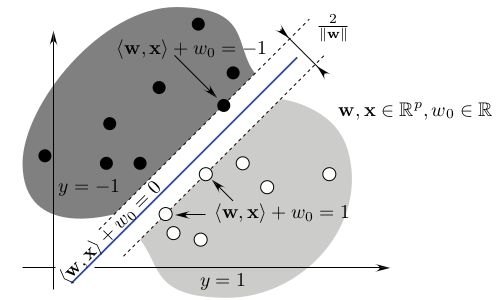
\includegraphics[scale=0.6]{SVM.png}
\end{center}

Three planes:

- $H_1: \omega^Tx+b=1$

- $H: \omega^Tx+b=0$

- $H_{-1}: \omega^Tx+b=-1$

\vspace{5mm}

Computing $H_1 - H_{-1}$ we get:

$(x_1-x_{-1})\omega^T=2$

=> $||x_1-x_{-1}||=\frac{2}{||\omega||}$

\vspace{5mm}

The SVM problem starts with a \textbf{margin maximization}. \textcolor{orange}{We want to maximize the distance between $x_1$ and $x_{-1}$ (\textbf{to be double checked})} and it is equivalent to minimizing $||\omega||$. Thus the optimization problem is written as such:

\begin{center}
$min_{\omega,b}~\frac{1}{2}||\omega||^2$

$s.t.~y_i(\omega^Tx_i+b) \geq 1$ $i=1,...,n$
\end{center}

\vspace{5mm}

\underline{Primal formulation}

\vspace{5mm}

The above problem reflects the case where all data are perfectly separable, this is not true in practice. We thus add an error term $\xi_i$ for each observation. This leads to the \textbf{primal formulation} of the problem:

\begin{center}
$min_{\omega,b, \xi}~\frac{1}{2}||\omega||^2+C\Sigma_{i=1}^{n}\xi_i$

$s.t.~y_i(\omega^Tx_i+b) \geq 1 - \xi_i$ $i=1,...,n$

$\xi_i \geq 0$ $i=1,...,n$
\end{center}

\vspace{5mm}

The problem is convex with lineary inequality constraints, we can apply the saddle point theorem.

\textit{Note}: a point is saddle if it's a maximum w.r.t. one axis and a minimium w.r.t. another axis 

\vspace{5mm}

\underline{Lagrange}

\vspace{5mm}

We can write this problem using Lagrange formulation, that is, integrating the constraints into the main formula:

$\mathcal{L}(\omega,b,\xi, \alpha, \mu) = \frac{1}{2}\omega^T\omega+C\Sigma \xi_i + \Sigma \alpha_i (1-\xi_i - y_i(\omega^Tx_i+b)) - \Sigma \mu_i \xi_i$

$\alpha_i, \mu_i \geq 0$

\vspace{5mm}

First order conditions:

$\frac{\partial\mathcal{L}}{\partial\omega} = 0 => \omega - \Sigma \alpha_i y_i x_i = 0 => \omega = \Sigma \alpha_i y_i x_i$

$\frac{\partial\mathcal{L}}{\partial b} = 0 => -\Sigma \alpha_i y_i = 0$

$\frac{\partial\mathcal{L}}{\partial \xi_i} = 0 => C - \alpha_i  - \mu_i = 0 => \alpha_i = C - \mu_i$

Since $\alpha_i, \mu_i \geq 0$ we have $C \geq \alpha_i \geq 0$

\vspace{5mm}

\underline{Dual formulation}

\vspace{5mm}

We can rewrite the problem using the first order conditions above:

$\mathcal{L}(\omega,b,\xi, \alpha, \mu) = \frac{1}{2}(\Sigma \alpha_i y_i x_i)^T(\Sigma \alpha_i y_i x_i)+C\Sigma \xi_i + \Sigma \alpha_i - \Sigma \alpha_i \xi_i - \Sigma \alpha_i y_i (\Sigma \alpha_i y_i x_i)^T x_i - \Sigma \alpha_i y_i b - \Sigma \mu_i \xi_i$

$~~~~~~~~~~~~~~~~~~ = -\frac{1}{2}(\Sigma \alpha_i y_i x_i)^T(\Sigma \alpha_i y_i x_i) + \Sigma(C - \alpha_i - \mu_i)\xi_i + \Sigma \alpha_i - \Sigma \alpha_i y_i b$

$~~~~~~~~~~~~~~~~~~ = -\frac{1}{2}\Sigma_{i,j} \alpha_i \alpha_j y_i y_j x_i^T x_j + \Sigma \alpha_i$

\vspace{5mm}

This leads to the problem in its \textbf{dual formulation}:

\begin{center}

$max_\alpha~~-\frac{1}{2}\Sigma_{i,j} \alpha_i \alpha_j y_i y_j x_i^T x_j + \Sigma \alpha_i$

$s.t.~~0 \leq \alpha_i \leq C~~i=1,...,n$

$\Sigma \alpha_i y_i = 0~~i=1,...,n$

\end{center}

\vspace{5mm}

Using the above expression of $\omega$ (optimal condition), the classification function is:

\begin{center}
$f(x)=sign(\Sigma \alpha_i y_i x_i^T x + b)$
\end{center}

\vspace{5mm}

\underline{Kernel}

\vspace{5mm}

Kernels are used when separation is non linear.

Recall the primal formulation:

\begin{center}
$min_{\omega,b, \xi}~\frac{1}{2}||\omega||^2+C\Sigma_{i=1}^{n}\xi_i$

$s.t.~y_i(\omega^Tx_i+b) \geq 1 - \xi_i$ $i=1,...,n$

$\xi_i \geq 0$ $i=1,...,n$
\end{center}

When separation is non linear, we set $\phi$ as a non linear transformation. The constraint becomes:

$y_i(\omega^T\phi(x_i)+b) \geq 1 - \xi_i~~i=1,...,n$

\vspace{5mm}

Dual formulation is now:

\begin{center}

$max_\alpha~~-\frac{1}{2}\Sigma_{i,j} \alpha_i \alpha_j y_i y_j \phi(x_i)^T \phi(x_j) + \Sigma \alpha_i$

$s.t.~~0 \leq \alpha_i \leq C~~i=1,...,n$

$\Sigma \alpha_i y_i = 0~~i=1,...,n$

\end{center}

\vspace{5mm}

The classification becomes:

\begin{center}
$f(x)=sign(\Sigma \alpha_i y_i \phi(x_i)^T \phi(x) + b)$
\end{center}

To classify a new point, we thus need to be able to compute $\phi(x_i)^T \phi(x)$.

\vspace{5mm}

\textbf{Kernel trick}: there is no need to know an explicit expression of $\phi$ (i.e. knowing the coordinates of points in new set) since we are only looking at distances and angles, that is scalar product.

\vspace{5mm}

Kernel functions implement those scalar products: $K(x,x')=\phi(x)^T \phi(x')$ where $\phi$ is a transformation function into a Hilbertian set $\phi : \mathcal{X} \to \mathcal{F} $

\textit{Note}: an Hilbertian is a set with scalar product: $\mathcal{F}=(\mathcal{H},<.,.>)$

\vspace{5mm}

Most used kernels:

Linear kernel: $K(x,x') = x^Tx'$ (we often call this setup a "no-kernel SVM")

Polynomial kernel: $K(x,x') = (x^Tx'+c)^d$

Gaussian kernel: $K(x,x') = exp(-\gamma||x-x'||^2)$

\vspace{5mm}

\underline{Summary}

\vspace{5mm}

SVM allows to find complex non linear separations in transforming the problem into a higher dimension where data are linearly separable.

\vspace{5mm}

From 1D to 2D:

\begin{center}
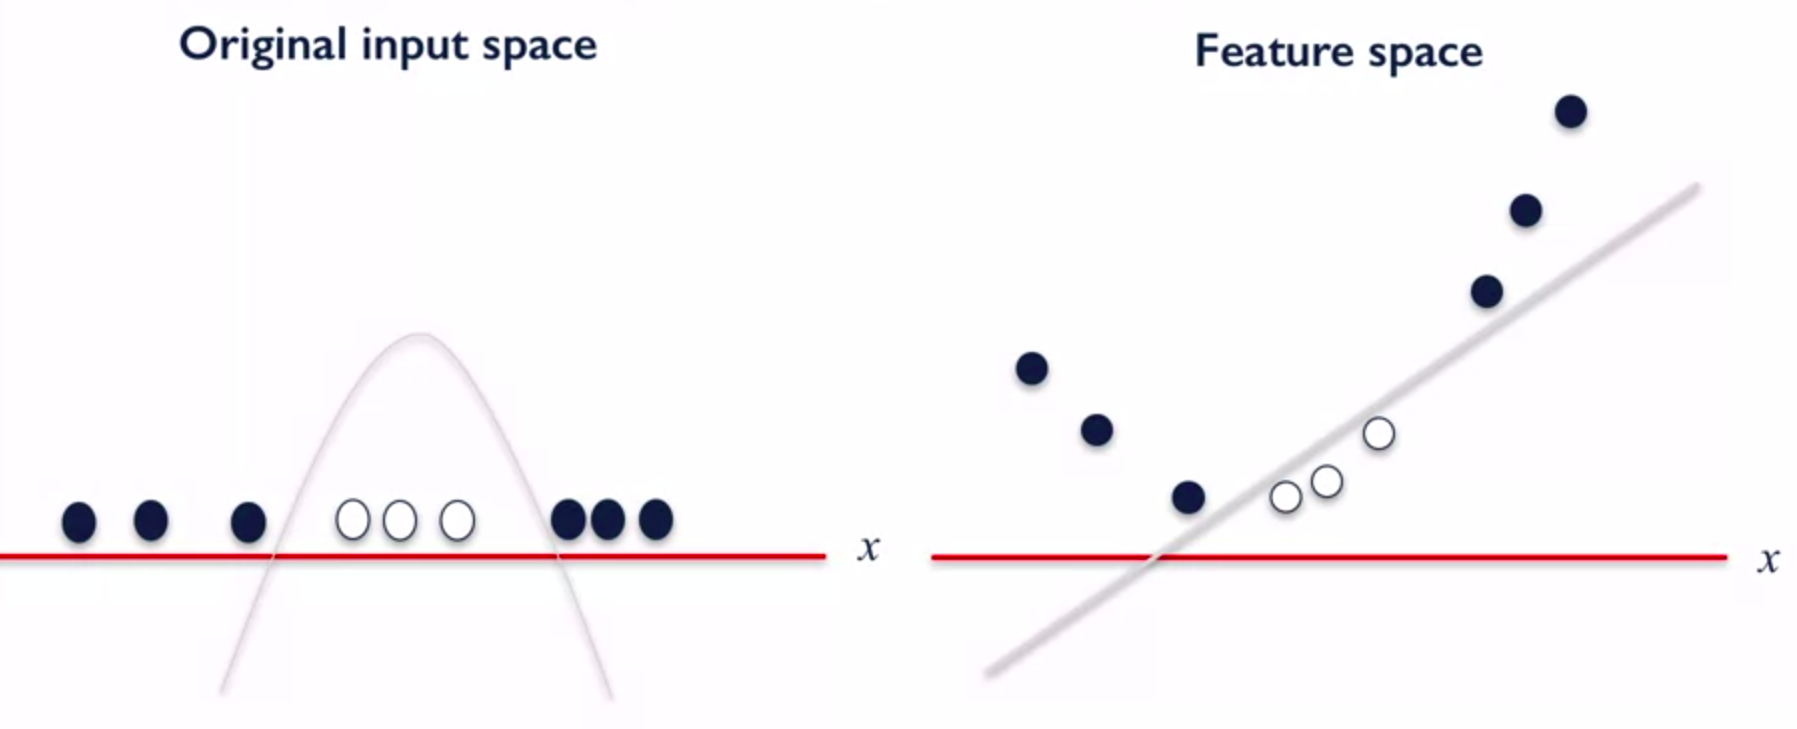
\includegraphics[scale=0.15]{kernel_2D.png}
\end{center}

\vspace{5mm}

From 2D to 3D:

\begin{center}
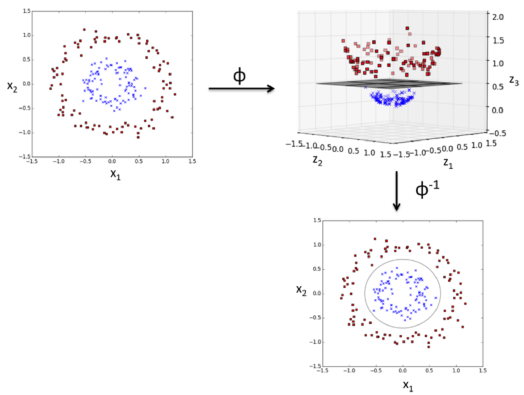
\includegraphics[scale=0.5]{kernel_3D.png}
\end{center}

\vspace{5mm}